\documentclass{tufte-handout}

\usepackage{graphicx,amsmath}

\title{Probability Distributions}
\author{M. Henry Linder}
\date{}

\begin{document}
\maketitle

\section{Binomial Distribution}
\begin{figure}
    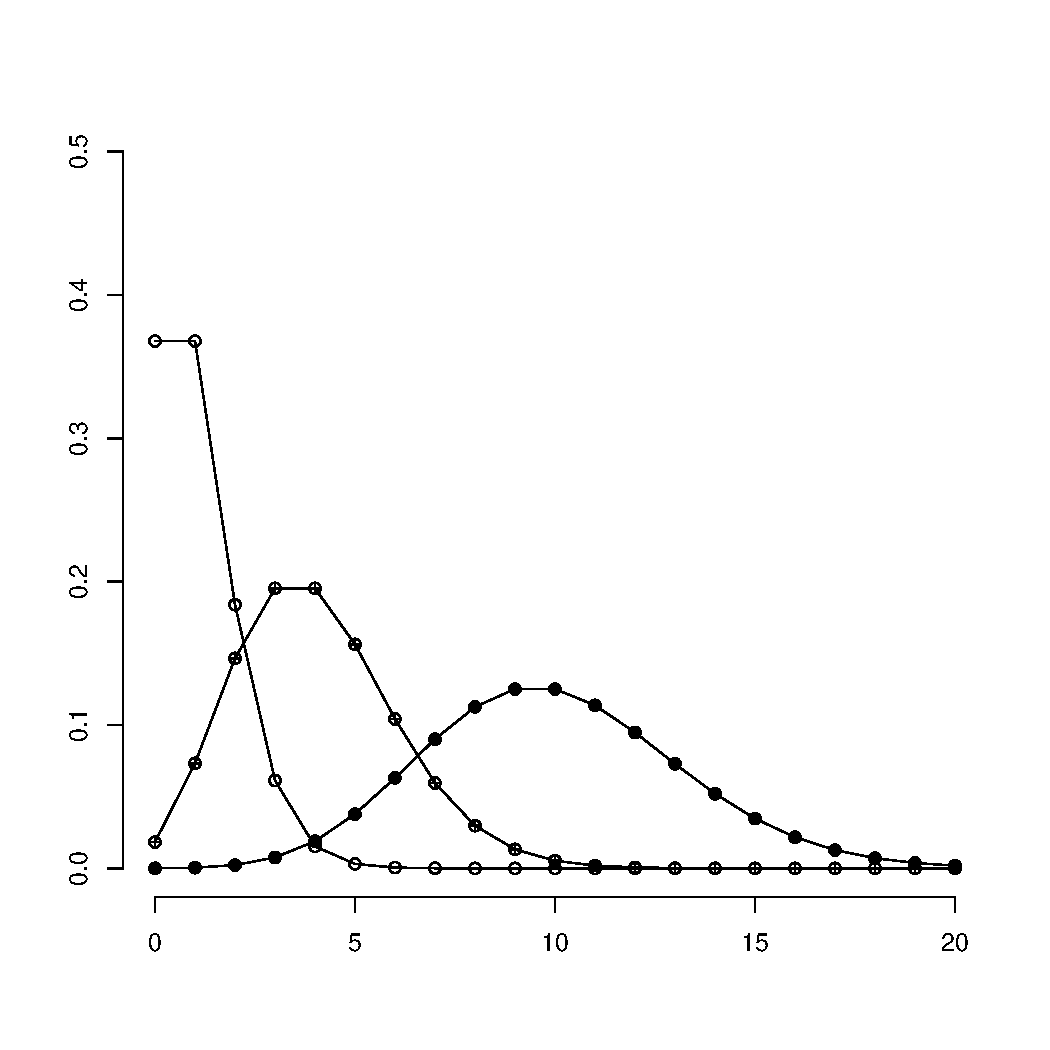
\includegraphics[width=\textwidth]{../distributions/poisson/poisson_bw.pdf}
    \caption{Binomial Distribution}
\end{figure}
\marginnote[-4.0in]{
    \begin{align*}
        & X \sim \text{Binomial} (n, p) \\
        & x = 0, 1, 2, \dots, n \\
        & 0 < p < 1 \\
        & p(x) = {n \choose x} p^x (1-p)^{x-1} \\
        & \mu = E[X] = np \\
        & \sigma^2 = E[(x-\mu)^2] = np(1-p) \\
    \end{align*}
}
\newpage

\section{Poisson Distribution}
\begin{figure}
    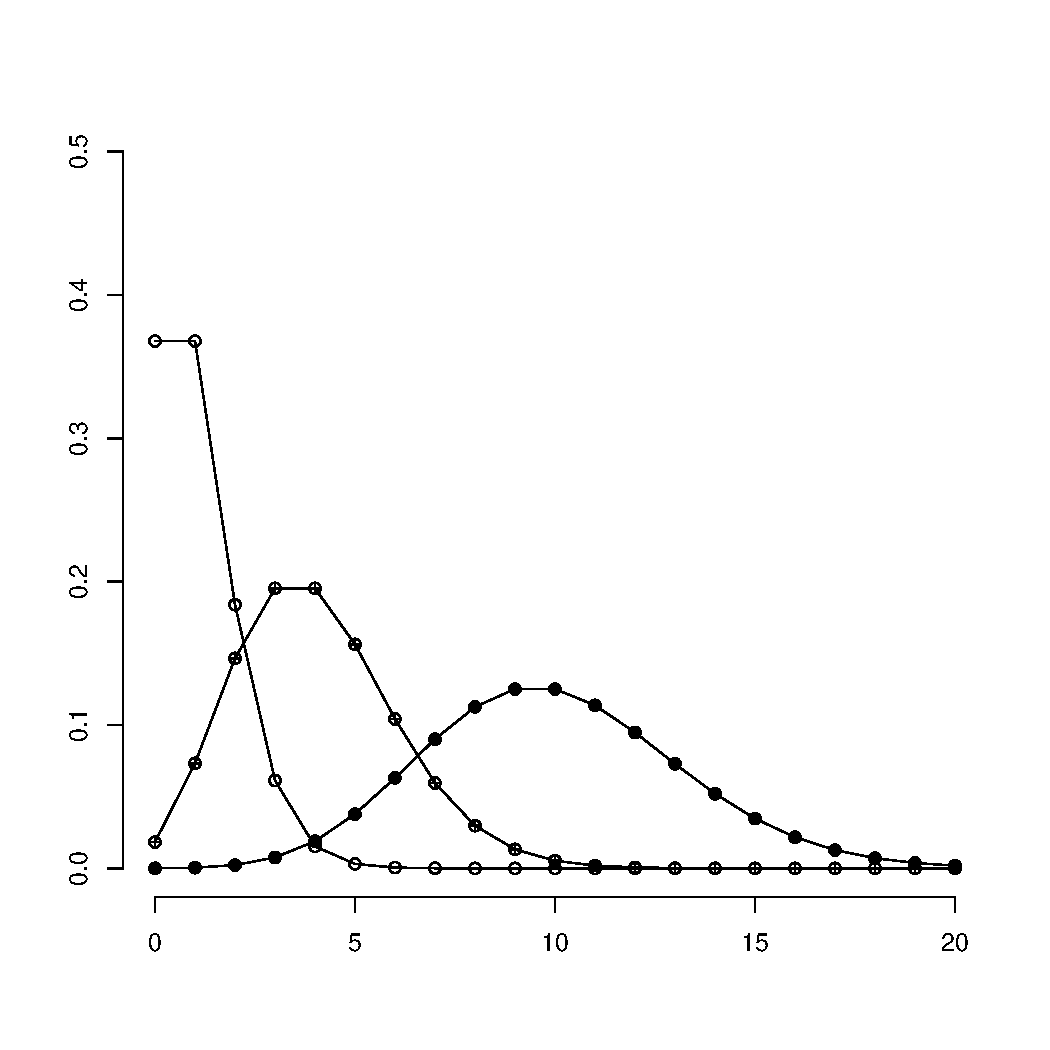
\includegraphics[width=\textwidth]{../distributions/poisson/poisson_bw.pdf}
    \caption{Poisson Distribution}
\end{figure}
\marginnote[-4.0in]{
    \begin{align*}
        & X \sim \text{Poisson} (\lambda) \\
        & x = 0, 1, 2, \dots \\
        & 0 < \lambda < \infty \\
        & p(x) = \frac{e^{-\lambda}\lambda^x}{x!} \\
        & \mu = E[X] = \lambda \\
        & \sigma^2 = E[(x-\mu)^2] = \lambda \\
    \end{align*}
}

\end{document}
